\documentclass[11pt,fleqn,report]{ltjsbook}

% 独自のスタイルファイルを読み込み
\usepackage{RSL_style}

% 画像パス設定 (main.texと同階層または上の階層の画像ディレクトリを参照可能にする)
% これにより,src/main.texから src/にある適当な画像を参照したり,あるいはsrc/../にある画像も参照可能にする
% ※ 将来的にmain.texをsrc/lualatex/main.tex等に移動した際にも常にsrc/figures/等を参照できるようにするため
\graphicspath{{./}{../}}

% importパッケージ使用
\usepackage{import}

% ヘッダー高さを適切に設定
\setlength{\headheight}{18pt}

% book用の設定調整
% chapterベースの番号設定に変更(styleで定義されたsectionベースを上書き)
\numberwithin{equation}{chapter} % 数式番号を章ごとにリセット
\numberwithin{figure}{chapter} % 図番号を章ごとにリセット
\numberwithin{table}{chapter} % 表番号を章ごとにリセット

% book用の数式番号スタイル設定
\renewcommand{\theequation}{\thechapter.\arabic{equation}}
\renewcommand{\thefigure}{\thechapter.\arabic{figure}} % 図番号のスタイル設定
\renewcommand{\thetable}{\thechapter.\arabic{table}} % 表番号のスタイル設定

% book用のマーク設定
\renewcommand{\chaptermark}[1]{\markboth{第\thechapter 章~#1}{}}
\renewcommand{\sectionmark}[1]{\markright{\thesection~#1}}

% 設定ここまで

\begin{document}

\frontmatter % タイトルと目次
\pagestyle{empty}

% タイトルページ
\begin{titlepage}
    \centering
    \vspace*{2cm}

    {\Huge\textbf{LaTeX論文テンプレート}}

    \vspace{1cm}

    {\Large サブタイトル}

    \vspace{2cm}

    {\large 著者名}

    \vspace{1cm}

    {\large 所属機関}

    \vfill

    {\large \today}

\end{titlepage}

\cleardoublepage


\tableofcontents

\mainmatter{} % 本文
\pagestyle{fancy}

\chapter{テスト章}

この章はテスト用の章です。数式、図、表の例を示します\cite{example}。

\section{数式の例}

数式を以下に示します:

\begin{equation}
    \label{eq:test}
    E = mc^2
\end{equation}

式\eqref{eq:test}はアインシュタインの質量エネルギー等価性を表します。

\section{図の例}

図の例を以下に示します:

\begin{figure}[H]
    \centering
    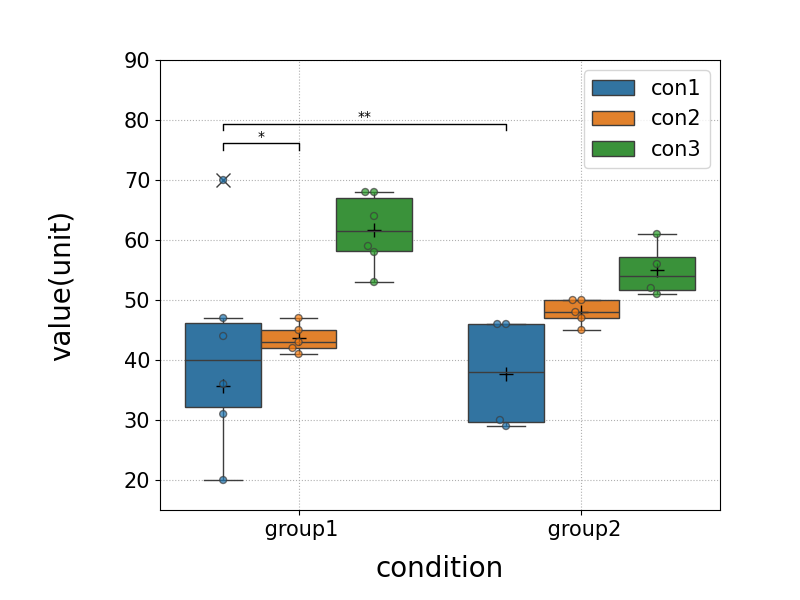
\includegraphics[width=0.8\textwidth]{figures/test/test.png} % サイズを指定
    \caption{テスト図}
    \label{fig:test}
\end{figure}

図\ref{fig:test}はテスト用の図です。

\section{表の例}

表の例を以下に示します:

\begin{table}[H]
    \centering
    \caption{テスト表}
    \label{tab:test}
    \begin{tabular}{|c|c|}
        \hline
        項目 & 値 \\
        \hline
        a & b \\
        c & d \\
        \hline
    \end{tabular}
\end{table}

表\ref{tab:test}はテスト用の表です。
 % テスト用の章

\chapter{はじめに}

本研究では,○○について検討する。

\section{研究背景}

近年,○○の分野において△△が注目されている。

\section{研究目的}

本研究の目的は以下の通りである:

\begin{itemize}
    \item ○○の効果を検証する
    \item △△の手法を提案する
    \item □□の性能を評価する
\end{itemize}

\section{本論文の構成}

本論文は以下のように構成されている:

\begin{description}
    \item[第1章] 研究の背景と目的について述べる
    \item[第2章] 関連研究について調査する
    \item[第3章] 提案手法について説明する
    \item[第4章] 実験結果について報告する
    \item[第5章] 結論と今後の課題について述べる
\end{description}

フォントテストも含める:

通常の明朝体: あいうえおABCabc123

{\sffamily ゴシック体: あいうえおABCabc123}

{\sffamily\bfseries ゴシック体太字: あいうえおABCabc123}


\bibliographystyle{unsrt} % 参考文献スタイル
\bibliography{reference} % 参考文献リストの表示

\end{document}
